\section{Specifica dei test}
\label{specifica}
Per produrre software di qualità, il gruppo SWEefty definirà dei test per assicurarsi che le unità prodotte funzionino in maniera corretta. Il tracciamento dei test ed il loro esito verrà riportato in questo documento.
	\subsection{Tipi di test}
	
		\subsubsection{Test di accettazione}
	Questi test vengono utilizzati durante il collaudo finale in presenza del committente.
	
	\newcolumntype{H}{>{\centering\arraybackslash}m{7cm}}
	\normalsize
	\begin{longtable}{|c|H|c|}
		\hline
		\textbf{Id Test} & \textbf{Descrizione} & \textbf{Stato}\\
		\hline
		\endhead
		TA0F1.1&L'utente intende visualizzare i componenti dell'applicazione sotto forma di mappa topologica. All'utente è richiesto di:\begin{itemize}
			\item premere sulla voce \emph{Mappa topologica} nel menù di \emph{Kibana}.
		\end{itemize}& \textcolor{green}{Superato} \\ \hline
		TA0F1.1.1&L'utente vuole verificare che vengano visualizzati nella mappa topologica i server dell'applicazione monitorata. All'utente è richiesto di:
		\begin{itemize}
			\item premere sulla voce \emph{Mappa topologica} nel menù di \emph{Kibana};
			\item verificare che i server vengano visualizzati.
		\end{itemize}& \textcolor{green}{Superato} \\ \hline
		TA0F1.1.2&L'utente intende verificare che vengano visualizzati nella mappa topologica i database dell'applicazione monitorata. All'utente è richiesto di:
		\begin{itemize}
			\item premere sulla voce \emph{Mappa topologica} nel menù di \emph{Kibana};
			\item verificare che i database vengano visualizzati.
		\end{itemize}& \textcolor{green}{Superato} \\ \hline
		TA1F1.1.3&L'utente intende verificare che vengano visualizzati nella mappa topologica i server cluster. All'utente e richiesto di:
		\begin{itemize}
			\item premere sulla voce \emph{Mappa topologica} nel menù di \emph{Kibana};
			\item verificare che i server cluster vengano visualizzati.
		\end{itemize}& \textcolor{red}{Non Superato} \\ \hline
		TA1F1.2&L'utente intende verificare che ogni tipologia di componente dell'applicazione monitorata venga rappresentata graficamente in modo diverso dalle altre. All'utente è richiesto di:
		\begin{itemize}
			\item premere sulla voce \emph{Mappa topologica} nel menù di \emph{Kibana};
			\item verificare che le varie componenti vengano visualizzate in modo diverso.
		\end{itemize}& \textcolor{green}{Superato} \\ \hline
		TA1F1.3&L'utente vuole verificare che vengano visualizzate le informazioni riguardanti i componenti dell'applicazione. All'utente è richiesto di:
		\begin{itemize}
			\item premere sulla voce \emph{Mappa topologica} nel menù di \emph{Kibana};
			\item verificare che vengano visualizzate le informazioni dei vari componenti.
		\end{itemize}& \textcolor{green}{Superato} \\ \hline
		TA1F1.4&L' utente vuole riposizionare i componenti all'interno della mappa topologica. All'utente è richiesto di:
		\begin{itemize}
			\item premere sulla voce \emph{Mappa topologica} nel menù di \emph{Kibana};
			\item cliccare e trascinare i vari componenti della mappa.
		\end{itemize}& \textcolor{green}{Superato} \\ \hline
		TA0F1.5&L'utente vuole verificare che venga visualizzato sotto forma di arco ciascun insieme di richieste fra due componenti della mappa. All'utente è richiesto di:
		\begin{itemize}
			\item premere sulla voce \emph{Mappa topologica} nel menù di \emph{Kibana};
			\item verificare che ciascun insieme di richieste fra due componenti sia visualizzato sotto forma di arco.
		\end{itemize}& \textcolor{green}{Superato} \\ \hline
		TA0F1.5.2.1&L'utente vuole verificare che venga visualizzato sotto forma di arco ciascun insieme di richieste fra un server ed un database. All'utente è richiesto di:
		\begin{itemize}
			\item premere sulla voce \emph{Mappa topologica} nel menù di \emph{Kibana};
			\item verificare che ciascun insieme di richieste fra un server ed un database venga visualizzato come un arco.
		\end{itemize}& \textcolor{green}{Superato} \\ \hline
		
		TA1F1.6&L'utente vuole verificare che vengano visualizzate informazioni sull'insieme di richieste fra due componenti dell'applicazione monitorata. All'utente è richiesto di:
		\begin{itemize}
			\item premere sulla voce \emph{Mappa topologica} nel menù di \emph{Kibana};
			\item verificare che vengano visualizzate informazioni su ciascun insieme di richieste fra due componenti.
		\end{itemize}& \textcolor{green}{Superato} \\ \hline
	
		TA1F1.6.1&L'utente vuole verificare che vengono visualizzati i tempi medi di risposta di ciascun insieme di richieste fra due componenti. All'utente è richiesto di:
		\begin{itemize}
			\item premere sulla voce \emph{Mappa topologica} nel menù di \emph{Kibana};
			\item verificare che vengano visualizzati i tempi medi di risposta.
		\end{itemize}& \textcolor{green}{Superato} \\ \hline
	
		TA1F1.6.2&L'utente vuole verificare che venga visualizzato sotto forma di etichetta il tipo dell'insieme di richieste fatte fra due componenti. All'utente è richiesto di:
		\begin{itemize}
			\item premere sulla voce \emph{Mappa topologica} nel menù di \emph{Kibana};
			\item verificare che vicino a ciascun arco ci sia un'etichetta che identifica il tipo dell'insieme di richieste.
		\end{itemize}& \textcolor{green}{Superato} \\ \hline
	
		TA1F1.8&L'utente vuole visualizzare un messaggio d'errore nel caso in cui ci sia un errore nel caricamento della mappa topologica. All'utente è richiesto di:
		\begin{itemize}
			\item premere sulla voce \emph{Mappa topologica} nel menù di \emph{Kibana} in assenza di connessione;
			\item verificare che venga visualizzato l'errore.
		\end{itemize}& \textcolor{green}{Superato} \\ \hline
	
		TA0F2&L'utente vuole visualizzare la lista delle tace dell'applicazione monitorata. All'utente viene chiesto di:
		\begin{itemize}
			\item cliccare sulla voce \emph{stack trace} nel menù di \emph{Kibana};
			\item verificare che la lista venga visualizzata correttamente.
		\end{itemize}& \textcolor{green}{Superato} \\ \hline
		TA0F2.1&L'utente vuole visualizzare i dettagli relativi ad una singola trace. All'utente è richiesto di:
		\begin{itemize}
			\item cliccare sulla voce \emph{stack trace} nel menù di \emph{Kibana};
			\item selezionare una trace cliccando due volte su di una riga;
			\item verificare che i dettagli vengano visualizzati correttamente.
		\end{itemize}&\textcolor{green}{Superato} \\ \hline
	
		TA1F2.1.1&L'utente vuole verificare che ogni voce nella lista delle trace sia numerata in modo incrementale a partire da 1. All'utente è richiesto di:
		\begin{itemize}
			\item cliccare sulla voce \emph{stack trace} nel menù di \emph{Kibana};
			\item verificare che le voci della lista siano numerate correttamente.
		\end{itemize}&\textcolor{green}{Superato} \\ \hline
		TA0F2.1.2&L'utente vuole verificare che per ogni voce della lista delle trace venga visualizzato l'identificativo ad essa associato corrispondente alla richiesta HTTP effettuata. All'utente è richiesto di:
		\begin{itemize}
			\item cliccare sulla voce \emph{stack trace} nel menù di \emph{Kibana};
			\item verificare che a ogni voce sia associato l'identificativo esatto.
		\end{itemize}& \textcolor{green}{Superato} \\ \hline
	
		TA1F2.1.3&L'utente vuole visualizzare data e ora di inizio di una trace. All'utente è richiesto di:
		\begin{itemize}
			\item cliccare sulla voce \emph{stack trace} nel menù di \emph{Kibana};
			\item verificare che sia presente la voce "timestamp" nella lista.
		\end{itemize}& \textcolor{green}{Superato} \\ \hline
		TA1F2.1.4&L'utente vuole visualizzare il tempo di esecuzione di una trace.All'utente è richiesto di:
		\begin{itemize}
			\item cliccare sulla voce \emph{stack trace} nel menù di    \emph{Kibana};
			\item verificare che sia presente la voce "execution time".
		\end{itemize}& \textcolor{green}{Superato} \\ \hline
		TA0F2.1.5&L'utente vuole visualizzare il codice di stato della richiesta HTTP corrispondente ad una trace. All'utente è richiesto di:
		\begin{itemize}
			\item cliccare sulla voce \emph{stack trace} nel menù di \emph{Kibana};
			\item verificare che il codice di stato della richiesta HTTP corrispondente ad una trace sia visualizzato correttamente.
		\end{itemize}& \textcolor{green}{Superato} \\ \hline
	
		TA1F2.2&L'utente vuole riordinare la lista delle trace. All'utente è richiesto di:
		\begin{itemize}
			\item cliccare sulla voce \emph{stack trace} nel menù di \emph{Kibana};
			\item cliccare sul titolo della colonna a seconda della quale si vogliono ordinare le trace.
		\end{itemize}& \textcolor{green}{Superato} \\ \hline
		TA0F2.3&L'utente vuole verificare che la lista delle trace sia inizialmente ordinata in modo decrescente rispetto all'ordine cronologico di esecuzione. All'utente è richiesto di:
		\begin{itemize}
			\item cliccare sulla voce \emph{stack trace} nel menù di \emph{Kibana};
			\item verificare che le trace siano nell'ordine corretto.
		\end{itemize}& \textcolor{green}{Superato} \\ \hline
		TA1F2.4&L'utente vuole verificare che nel caso ci sia un errore nel caricamento dei dati della lista delle trace venga visualizzato un messaggio d'errore. All'utente è richiesto di:
		\begin{itemize}
			\item cliccare sulla voce \emph{stack trace} nel menù di \emph{Kibana} senza una connessione al database;
			\item verificare che venga visualizzato il messaggio d'errore.
		\end{itemize}& \textcolor{green}{Superato} \\ \hline
		TA0F3&L'utente vuole visualizzare il call tree di una trace. All'utente è richiesto di:
		\begin{itemize}
			\item cliccare sulla voce \emph{stack trace} nel menù di \emph{Kibana};
			\item cliccare sulla riga della trace di cui si vuole avere il call tree;
			\item verificare che il call tree venga visualizzato correttamente.
		\end{itemize}& \textcolor{green}{Superato} \\ \hline
		TA0F3.1&L'utente vuole visualizzare i dettagli ogni singolo metodo di una trace. All'utente è richiesto di:
		\begin{itemize}
			\item cliccare sulla voce \emph{stack trace} nel menù di \emph{Kibana};
			\item cliccare sulla riga della trace di cui si vogliono conoscere i dettagli sui metodi;
			\item verificare che vengano visualizzati i dettagli sui metodi.
		\end{itemize}& \textcolor{green}{Superato} \\ \hline
		TA0F3.1.1&L'utente vuole visualizzare il nome di ogni singolo metodo invocato all'interno di una trace. All'utente è richiesto di:
		\begin{itemize}
			\item cliccare sulla voce \emph{stack trace} nel menù di \emph{Kibana};
			\item cliccare sulla riga della trace di cui si vogliono conoscere i nomi dei metodi;
			\item verificare che vengano visualizzati i nomi dei metodi.
		\end{itemize}& \textcolor{green}{Superato} \\ \hline
		TA1F3.1.2&L'utente vuole visualizzare il self execution time di un metodo. All'utente è richiesto di:
		\begin{itemize}
			\item cliccare sulla voce \emph{stack trace} nel menù di \emph{Kibana};
			\item cliccare sulla riga della trace che contiene il metodo di cui si vuole conoscere il self execution time;
			\item verificare che venga visualizzato il self execution time del metodo.
		\end{itemize}& \textcolor{green}{Superato} \\ \hline
		TA1F3.1.3&L'utente vuole visualizzare il total execution time di un metodo. All'utente è richiesto di:
		\begin{itemize}
			\item cliccare sulla voce \emph{stack trace} nel menù di \emph{Kibana};
			\item cliccare sulla riga della trace che contiene il metodo di cui si vuole conoscere il total execution time;
			\item verificare che venga visualizzato il total execution time del metodo.
		\end{itemize}& \textcolor{green}{Superato} \\ \hline
		TA1F3.4&L'utente vuole verificare che al momento del caricamento vengano visualizzate tutte le sottochiamate di ogni metodo. All'utente è richiesto di:
		\begin{itemize}
			\item cliccare sulla voce \emph{stack trace} nel menù di \emph{Kibana};
			\item verificare che vengano visualizzate tutte le sottochiamate di ogni metodo.
		\end{itemize}& \textcolor{green}{Superato} \\ \hline
	
		TA1F4&L'utente vuole visualizzare la lista delle query eseguite in una singola trace. All' utente è richiesto di:
		\begin{itemize}
			\item cliccare sulla voce \emph{stack trace} nel menù di \emph{Kibana};
			\item cliccare sulla riga della trace di interesse;
			\item cliccare sulla voce "query list"
			\item verificare che venga visualizzata la lista delle query eseguite.
		\end{itemize}& \textcolor{green}{Superato} \\ \hline
		TA1F4.1&L'utente vuole visualizzare dei dettagli riguardanti una singola query. All'utente è richiesto di:
		\begin{itemize}
			\item cliccare sulla voce \emph{stack trace} nel menù di \emph{Kibana};
			\item cliccare sulla riga della trace di interesse;
			\item cliccare sulla voce "query list"
			\item verificare che vengano visualizzati i dettagli di ogni singola query.
		\end{itemize}& \textcolor{green}{Superato} \\ \hline
	
		TA1F4.2&L'utente vuole riordinare la lista delle query relativa ad una singola trace. All'utente è richiesto di:
		\begin{itemize}
			\item cliccare sulla voce \emph{stack trace} nel menù di \emph{Kibana};
			\item cliccare sulla riga della trace di interesse;
			\item cliccare sulla voce "query list"
			\item cliccare sul titolo della colonna a seconda della quale si vogliono ordinare le query.
		\end{itemize}&\textcolor{green}{Superato} \\ \hline
		TA1F4.3&L'utente vuole verificare che la lista delle query in una singola trace venga inizialmente visualizzata in ordine decrescente rispetto all'ordine cronologico di esecuzione. All'utente è richiesto di:
		\begin{itemize}
			\item cliccare sulla voce \emph{stack trace} nel menù di \emph{Kibana};
			\item cliccare sulla riga della trace di interesse;
			\item cliccare sulla voce "query list"
			\item verificare che la lista delle query sia nell'ordine giusto.
		\end{itemize}& \textcolor{green}{Superato} \\ \hline
	\end{longtable}
	
	\begin{figure}[H]
		\centering 
		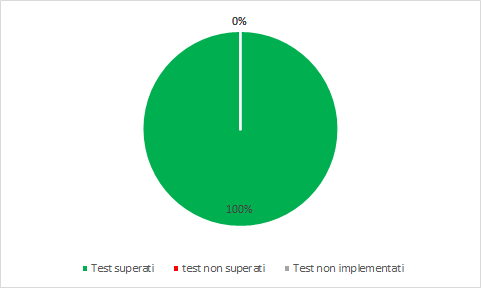
\includegraphics[width=0.6\textwidth]{Images/TA.png}
		\caption{Sintesi della percentuale di test di accettazione superati}
		\label{TA} 
	\end{figure}	
	
	\paragraph{Tracciamento} \Spazio
	
	\begin{longtable}{|c|c|}
		\hline
		\textbf{Id Test} & \textbf{Id Requisito}\\
		\hline
		\endhead
		TA0F1.1&R0F1.1 \\ \hline
		TA0F1.1.1&R0F1.1.1 \\ \hline
		TA0F1.1.2&R0F1.1.2 \\ \hline
		TA1F1.1.3&R1F1.1.3 \\ \hline
		TA1F1.2&R1F1.2 \\ \hline
		TA1F1.3&R1F1.3 \\ \hline
		TA1F1.4&R1F1.4 \\ \hline
		TA0F1.5&R0F1.5 \\ \hline
		TA0F1.5.2.1&R0F1.5.2.1 \\ \hline
		TA0F1.5.2.2&R0F1.5.2.2 \\ \hline
		TA1F1.6&R1F1.6 \\ \hline
		TA1F1.6.1&R1F1.6.1 \\ \hline
		TA1F1.6.2&R1F1.6.2 \\ \hline
		TA1F1.8&R1F1.8 \\ \hline
		TA0F2&R0F2 \\ \hline
		TA0F2.1&R0F2.1 \\ \hline
		TA1F2.1.1&R1F2.1.1 \\ \hline
		TA0F2.1.2&R0F2.1.2 \\ \hline
		TA1F2.1.3&R1F2.1.3 \\ \hline
		TA1F2.1.4&R1F2.1.4 \\ \hline
		TA0F2.1.5&R0F2.1.5 \\ \hline
		TA1F2.2&R1F2.2 \\ \hline
		TA0F2.3&R0F2.3 \\ \hline
		TA1F2.4&R1F2.4 \\ \hline
		TA0F3&R0F3 \\ \hline
		TA0F3.1&R0F3.1 \\ \hline
		TA0F3.1.1&R0F3.1.1 \\ \hline
		TA1F3.1.2&R1F3.1.2 \\ \hline
		TA1F3.1.3&R1F3.1.3 \\ \hline
		TA1F3.4&R1F3.4 \\ \hline
		TA1F4&R1F4 \\ \hline
		TA1F4.1&R1F4.1 \\ \hline
		TA1F4.2&R1F4.2 \\ \hline
		TA1F4.3&R1F4.3 \\ \hline
	\end{longtable}

    \subsubsection{Test di sistema}
    Questo tipo di test serve per verificare che il comportamento dinamico del sistema sia conforme ai requisiti specificati nel documento \textit{Analisi dei Requisiti\_v4.0.0}.
    \begin{longtable}{|c|H|c|}
    	\hline
    	\textbf{Id Test} & \textbf{Descrizione} & \textbf{Stato}\\
    	\hline
    	\endhead
    	TS0F1.1&Viene verificato che sia possibile visualizzare le varie componenti del sistema.& \textcolor{green}{Superato}\\ \hline
    	TS0F1.1.1&Vene verificato che sia possibile visualizzare i server nella mappa.&\textcolor{green}{Superato} \\ \hline
    	TS0F1.1.2&Viene verificato che sia possibile visualizzare nella mappa i database dell'applicazione monitorata.&\textcolor{green}{Superato} \\ \hline
    	TS1F1.1.3&Viene verificato che sia possibile visualizzare nella mappa i server cluster dell'applicazione monitorata.&\textcolor{red}{Non Superato} \\ \hline
    	TS1F1.2&Viene verificato che ogni componente dell'applicazione venga visualizzato in modo differente.&Non implementato \\ \hline
    	TS1F1.2.1&Viene verificato che i server siano rappresentati sotto forma di cerchi.&\textcolor{green}{Superato} \\ \hline
    	TS1F1.2.2&Viene verificato che i database siano rappresentati sotto forma di cilindri.&\textcolor{green}{Superato} \\ \hline
    	TS1F1.2.3&Viene verificato che sia possibile visualizzare il numero di server che compongono un cluster.&\textcolor{red}{Non Superato} \\ \hline
    	TS1F1.3&Viene verificato che sia possibile visualizzare le informazioni riguardanti i componenti della mappa topologica dell'applicazione.&\textcolor{green}{Superato} \\ \hline
    	TS2F1.3.1&Viene verificato che sia possibile visualizzare il linguaggio d'implementazione dei server tramite un rettangolo informativo vicino al componente.&\textcolor{red}{Non Superato} \\ \hline
    	TS1F1.3.2&Viene verificato che sia possibile visualizzare vicino ad ogni componente dell'applicazione monitorata un identificativo per tale entità.&\textcolor{green}{Superato} \\ \hline
    	TS1F1.4&Viene verificato ch l'utente possa riposizionare i componenti all'interno della mappa topologica.&\textcolor{green}{Superato} \\ \hline
    	TS2F1.4.1&Viene verificato che sia possibile riposizionare ogni componente della mappa trascinando con il puntatore.&\textcolor{green}{Superato} \\ \hline
    	TS2F1.4.2&Viene verificato che sia possibile riposizionare automaticamente i componenti all'interno della mappa.&\textcolor{green}{Superato} \\ \hline
    	TS0F1.5&Viene verificato che sia possibile visualizzare ciascun insieme di richieste fra due componenti della mappa topologica sotto forma di arco tra i due.&\textcolor{green}{Superato} \\ \hline
    	TS2F1.5.1&Viene verificato che il colore degli archi cambi in base al tempo medio di un insieme di richieste fra due componenti dell'applicazione monitorata.&\textcolor{green}{Superato} \\ \hline
    	TS2F1.5.1.1&Viene verificato che se il tempo di esecuzione medio di un insieme di richieste fra due componenti dell'applicazione monitorata sale oltre i 3 secondi l'arco che li unisce diventi rosso.&\textcolor{green}{Superato} \\ \hline
    	TS2F1.5.1.2&Viene verificato che se il tempo di esecuzione medio di un
    	insieme di richieste fra due componenti dell'applicazione monitorata è inferiore o uguale a 3 secondi l'arco che li unisce sia nero.&\textcolor{green}{Superato} \\ \hline
    	TS0F1.5.2&Viene verificato che sia possibile visualizzare gli archi in base al tipo di richiesta eseguita fra due componenti della mappa topologica.&\textcolor{green}{Superato} \\ \hline
    	TS0F1.5.2.1&Viene verificato che sia possibile visualizzare sotto forma di arco un insieme di richieste fra un server e un database.&\textcolor{green}{Superato} \\ \hline
    	TS0F1.5.2.2&Viene verificato che sia possibile visualizzare sotto forma di arco un insieme di richieste HTTP fra due server.&\textcolor{green}{Superato} \\ \hline
    	TS1F1.6&Viene verificato che sia possibile visualizzare informazioni sull'insieme di richieste fra due componenti dell'applicazione.&\textcolor{green}{Superato} \\ \hline
    	TS1F1.6.1&Viene verificato che sia possibile visualizzare il tempo medio di risposta di un insieme di richieste fra due componenti dell'applicazione monitorata.&\textcolor{green}{Superato} \\ \hline
    	TS1F1.6.2&Viene verificato che sia possibile visualizzare sotto forma di etichetta il tipo dell'insieme di richieste fatte fra due componenti.&\textcolor{green}{Superato} \\ \hline
    	TS1F1.6..2.1&Viene verificato che sia possibile visualizzare delle etichette con la scritta "DB" sugli archi che presentano delle richieste fra server e database.&\textcolor{green}{Superato} \\ \hline
    	TS1F1.6.2.2&Viene verificato che sia possibile visualizzare delle etichette con la scritta "HTTP" sugli archi che rappresentano delle richieste HTTP fra server e server.&\textcolor{green}{Superato} \\ \hline
    	TS2F1.7&Viene verificato che sia possibile ridimensionare la grandezza della mappa topologica.&\textcolor{green}{Superato} \\ \hline
    	TS2F1.7.1&Viene verificato che sia possibile ingrandire i componenti della mappa topologica.&\textcolor{green}{Superato} \\ \hline
    	TS2F1.7.2&Viene verificato che sia possibile restringere la dimensione dei componenti della mappa.&\textcolor{green}{Superato} \\ \hline
    	TS2F1.7.3&Viene verificato che sia possibile visualizzare la mappa topologica in modalità a schermo intero.&\textcolor{green}{Superato} \\ \hline
    	TS1F1.8&Viene verificato che nel caso in cui ci sia un errore nel caricamento dei dati della mappa topologica venga visualizzato un messaggio d'errore. &\textcolor{green}{Superato} \\ \hline
    	TS0F2&Viene verificato che sia possibile visualizzare una lista delle trace dell'applicazione monitorata.&\textcolor{green}{Superato} \\ \hline
    	TS0F2.1&Viene verificato che sia possibile visualizzare i dettagli relativi ad ogni singola trace.&\textcolor{green}{Superato} \\ \hline
    	TS1F2.1.1&Viene verificato che sia possibile visualizzare ogni voce nella lista delle trace associata ad un numero univoco incrementale.&\textcolor{green}{Superato} \\ \hline
    	TS0F2.1.2&Viene verificato che sia possibile visualizzare per ogni voce della lista delle trace l’identificativo ad essa associato corrispondente alla richiesta HTTP effettuata. &\textcolor{green}{Superato} \\ \hline
    	TS1F2.1.3&Viene verificato che sia possibile visualizzare data e orario del momento in cui è iniziata l'esecuzione di ogni trace. &\textcolor{green}{Superato} \\ \hline
    	TS1F2.1.4&Viene verificato che sia possibile visualizzare il tempo di esecuzione di ogni trace. &\textcolor{green}{Superato} \\ \hline
    	TS1F2.1.5&Viene verificato che sia possibile visualizzare il codice di stato della richiesta HTTP corrispondente ad ogni singola trace della lista.&\textcolor{green}{Superato} \\ \hline
    	TS1F2.1.5.1&Viene verificato che sia possibile visualizzare il dettaglio dell'errore avvenuto in forma testuale. &\textcolor{green}{Superato} \\ \hline
    	TS1F2.2&Viene verificato che sia possibile riordinare la lista delle trace. &\textcolor{green}{Superato} \\ \hline
    	TS1F2.2.1&Viene verificato che sia possibile riordinare la lista delle trace in base all'ordine cronologico di esecuzione. &\textcolor{green}{Superato} \\ \hline
    	TS1F2.2.1.1&Viene verificato che sia possibile riordinare la lista delle trace in base all'ordine cronologico di esecuzione in modo crescente. &\textcolor{green}{Superato} \\ \hline
    	TS1F2.2.1.2&Viene verificato che sia possibile riordinare la lista delle trace in base all'ordine cronologico di esecuzione in modo decrescente. &\textcolor{green}{Superato} \\ \hline
    	TS1F2.2.2&Viene verificato che sia possibile riordinare la lista delle trace in base al tempo di esecuzione. &\textcolor{green}{Superato} \\ \hline
    	TS1F2.2.2.1&Viene verificato che sia possibile riordinare la lista delle trace in base al tempo di esecuzione in modo crescente. &\textcolor{green}{Superato} \\ \hline
    	TS1F2.2.2.2&Viene verificato che sia possibile riordinare la lista delle trace in base al tempo di esecuzione in modo decrescente. &\textcolor{green}{Superato} \\ \hline
    	TS0F2.3&Viene verificato che la lista delle trace sia caricata in ordine decrescente rispetto all'ordine cronologico di esecuzione. &\textcolor{green}{Superato} \\ \hline
    	TS1F2.4&Viene verificato che sia visualizzato un messaggio di errore nel caso in cui ci sia un errore nel caricamento dei dati della lista delle trace.&\textcolor{green}{Superato} \\ \hline
    	TS0F3&Viene verificato che sia possibile visualizzare il call tree di ogni trace. &\textcolor{green}{Superato} \\ \hline
    	TS0F3.1&Viene verificato che sia possibile visualizzare dei dettagli riguardati ogni singolo metodo. &\textcolor{green}{Superato} \\ \hline
    	TS0F3.1.1&Viene verificato che sia possibile, per ogni metodo invocato, visualizzarne il nome. &\textcolor{green}{Superato} \\ \hline
    	TS1F3.1.2&Viene verificato che sia possibile, per ogni metodo invocato, visualizzare il self execution time.&\textcolor{green}{Superato} \\ \hline
    	TS1F3.1.3&Viene verificato che sia possibile, per ogni metodo invocato, visualizzare il total execution time.&\textcolor{green}{Superato} \\ \hline
    	TS2F3.1.4&Viene verificato che sia possibile,per ogni metodo invocato, visualizzare le query da esso effettuate.&\textcolor{green}{Superato} \\ \hline
    	TS2F3.2&Viene verificato che sia possibile raggruppare gerarchicamente le sottochiamate di un metodo del call tree. &\textcolor{green}{Superato} \\ \hline
    	TS2F3.2.1&Viene verificato che sia possibile nascondere le sottochiamate eseguite dal metodo. &\textcolor{green}{Superato} \\ \hline
    	TS1F3.2.2&Viene verificato che sia possibile visualizzare le sottochiamate eseguite dal metodo. &\textcolor{green}{Superato} \\ \hline
    	TS1F3.3&Viene verificato che Ogni livello di annidamento delle sottochiamate nel call tree deve avere essere mostrato con un livello di indentazione rispetto al precedente. &\textcolor{green}{Superato} \\ \hline
    	TS1F3.4&Viene verificato che al momento del caricamento tutte le sottochiamate di un call tree devono essere visualizzate.&Non implementato\\ \hline
    	TS1F4&Viene verificato che sia possibile visualizzare la lista delle query eseguite in una singola trace. &\textcolor{green}{Superato} \\ \hline
    	TS1F4.1&Viene verificato che sia possibile visualizzare dei dettagli riguardati ogni singola query.&\textcolor{green}{Superato} \\ \hline
    	TS1F4.1.1&Viene verificato che sia possibile visualizzare ogni voce nella lista delle query associata ad un numero univoco incrementale. &\textcolor{green}{Superato} \\ \hline
    	TS1F4.1.2&Viene verificato che sia possibile visualizzare il testo di tutte le query di una singola trace.&\textcolor{green}{Superato} \\ \hline
    	TS1F4.1.3&Viene verificato che sia possibile visualizzare l'identificativo del database interrogato da ogni query.&\textcolor{green}{Superato} \\ \hline
    	TS1F4.1.4&Viene verificato che sia possibile visualizzare data e orario del momento in cui è iniziata l' esecuzione di ogni query.&\textcolor{green}{Superato} \\ \hline
    	TS1F4.1.5&Viene verificato che sia possibile visualizzare il tempo di esecuzione di ogni query. &\textcolor{green}{Superato} \\ \hline
    	TS1F4.2&Viene verificato che sia possibile riordinare la lista delle query relativa ad una singola trace. &\textcolor{green}{Superato} \\ \hline
    	TS1F4.2.1&Viene verificato che sia possibile riordinare la lista delle query di una singola trace in base all'ordine cronologico di esecuzione. &\textcolor{green}{Superato} \\ \hline
    	TS1F4.2.1.1&Viene verificato che sia possibile riordinare la lista delle query di una singola trace in base all'ordine cronologico di esecuzione in modo crescente. &\textcolor{green}{Superato} \\ \hline
    	TS1F4.2.1.2&Viene verificato che sia possibile riordinare la lista delle query di una singola trace in base all'ordine cronologico di esecuzione in modo decrescente. &\textcolor{green}{Superato} \\ \hline
    	TS1F4.2.2&Viene verificato che sia possibile riordinare la lista delle query di una singola trace in base al tempo di esecuzione. &\textcolor{green}{Superato} \\ \hline
    	TS1F4.2.2.1&Viene verificato che sia possibile riordinare la lista delle query di una singola trace in base al tempo di esecuzione in modo crescente. &\textcolor{green}{Superato} \\ \hline
    	TS1F4.2.2.2&Viene verificato che sia possibile riordinare la lista delle query di una singola trace in base al tempo di esecuzione in modo decrescente. &\textcolor{green}{Superato} \\ \hline
    	TS1F4.3&Viene verificato che la lista delle query di una singola trace sia caricata in ordine decrescente rispetto all'ordine cronologico di esecuzione. &\textcolor{green}{Superato} \\ \hline
    	
    	TS0V3&Viene verificato che il prodotto sia compatibile con il browser Google Chrome v. 55.x.  &Non implementato \\ \hline
    	TS0V4&Viene verificato che il prodotto sia compatibile con il browser Mozilla Firefix v. 50.x. &Non implementato \\ \hline
    	TS0V5&Viene verificato che il prodotto sia compatibile con il browser Safari v. 10.x.&Non implementato \\ \hline
    	TS0V6&Viene verificato che il prodotto sia compatibile con il browser Internet Explorer v. 11.x.&Non implementato \\ \hline
    \end{longtable}


\begin{figure}[H]
\centering 
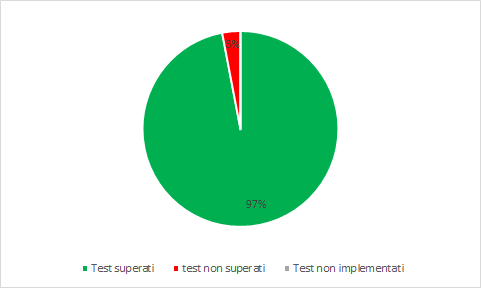
\includegraphics[width=0.6\textwidth]{Images/TS.png}
\caption{Sintesi della percentuale di test di sistema superati}
\label{TS} 
\end{figure}
    
    \paragraph{Tracciamento} \Spazio
    
    \begin{longtable}{|c|c|}
    	\hline
    	\textbf{Id Test} & \textbf{Id Requisito}\\
    	\hline
    	\endhead
    	TS0F1.1&R0F1.1\\ \hline
    	TS0F1.1.1&R0F1.1.1 \\ \hline
    	TS0F1.1.2&R0F1.1.2 \\ \hline
    	TS1F1.1.3&R1F1.1.3 \\ \hline
    	TS1F1.2&R1F1.2 \\ \hline
    	TS1F1.2.1&R1F1.2.1 \\ \hline
    	TS1F1.2.2&R1F1.2.2 \\ \hline
    	TS1F1.2.3&R1F1.2.3 \\ \hline
    	TS1F1.3&R1F1.3 \\ \hline
    	TS2F1.3.1&R2F1.3.1 \\ \hline
    	TS1F1.3.2&R1F1.3.2 \\ \hline
    	TS1F1.4&R1F1.4 \\ \hline
    	TS2F1.4.1&R2F1.4.1 \\ \hline
    	TS2F1.4.2&R2F1.4.2 \\ \hline
    	TS0F1.5&R0F1.5 \\ \hline
    	TS2F1.5.1&R2F1.5.1 \\ \hline
    	TS2F1.5.1.1&R2F1.5.1.1 \\ \hline
    	TS2F1.5.1.2&R2F1.5.1.2 \\ \hline
    	TS0F1.5.2&R0F1.5.2 \\ \hline
    	TS0F1.5.2.2&R0F1.5.2.2 \\ \hline
    	TS1F1.6&R1F1.6 \\ \hline
    	TS1F1.6.1&R1F1.6.1 \\ \hline
    	TS1F1.6.2&R1F1.6.2 \\ \hline
    	TS1F1.6..2.1&R1F1.6..2.1 \\ \hline
    	TS1F1.6.2.2&R1F1.6.2.2 \\ \hline
    	TS2F1.7&R2F1.7 \\ \hline
    	TS2F1.7.1&R2F1.7.1 \\ \hline
    	TS2F1.7.2&R2F1.7.2 \\ \hline
    	TS2F1.7.3&R2F1.7.3 \\ \hline
    	TS1F1.8&R1F1.8 \\ \hline
    	TS0F2&R0F2 \\ \hline
    	TS0F2.1&R0F2.1 \\ \hline
    	TS1F2.1.1&R1F2.1.1 \\ \hline
    	TS0F2.1.2&R0F2.1.2 \\ \hline
    	TS1F2.1.3&R1F2.1.3 \\ \hline
    	TS1F2.1.4&R1F2.1.4 \\ \hline
    	TS1F2.1.5&R1F2.1.5 \\ \hline
    	TS1F2.1.5.1&R1F2.1.5.1 \\ \hline
    	TS1F2.2&R1F2.2 \\ \hline
    	TS1F2.2.1&R1F2.2.1 \\ \hline
    	TS1F2.2.1.1&R1F2.2.1.1 \\ \hline
    	TS1F2.2.1.2&R1F2.2.1.2 \\ \hline
    	TS1F2.2.2&R1F2.2.2 \\ \hline
    	TS1F2.2.2.1&R1F2.2.2.1 \\ \hline
    	TS1F2.2.2.2&R1F2.2.2.2 \\ \hline
    	TS0F2.3&R0F2.3 \\ \hline
    	TS1F2.4&R1F2.4 \\ \hline
    	TS0F3&R0F3 \\ \hline
    	TS0F3.1&R0F3.1 \\ \hline
    	TS0F3.1.1&	R0F3.1.1 \\ \hline
    	TS1F3.1.2&R1F3.1.2 \\ \hline
    	TS1F3.1.3&R1F3.1.3 \\ \hline
    	TS2F3.1.4&R2F3.1.4 \\ \hline
    	TS2F3.2&R2F3.2 \\ \hline
    	TS2F3.2.1&R2F3.2.1 \\ \hline
    	TS1F3.2.2&R1F3.2.2 \\ \hline
    	TS1F3.3&R1F3.3 \\ \hline
    	TS1F3.4&R1F3.4\\ \hline
    	TS1F4&R1F4 \\ \hline
    	TS1F4.1&R1F4.1 \\ \hline
    	TS1F4.1.1&R1F4.1.1 \\ \hline
    	TS1F4.1.2&R1F4.1.2 \\ \hline
    	TS1F4.1.3&R1F4.1.3 \\ \hline
    	TS1F4.1.4&R1F4.1.4 \\ \hline
    	TS1F4.1.5&R1F4.1.5 \\ \hline
    	TS1F4.2&R1F4.2 \\ \hline
    	TS1F4.2.1&R1F4.2.1 \\ \hline
    	TS1F4.2.1.1&R1F4.2.1.1 \\ \hline
    	TS1F4.2.1.2&R1F4.2.1.2 \\ \hline
    	TS1F4.2.2&R1F4.2.2 \\ \hline
    	TS1F4.2.2.1&R1F4.2.2.1 \\ \hline
    	TS1F4.2.2.2&R1F4.2.2.2 \\ \hline
    	TS1F4.3&R1F4.3 \\ \hline
    	
    	TS0Q1&R0Q1 \\ \hline
    	TS0Q2&R0Q2 \\ \hline
    	TS0Q3&R0Q3 \\ \hline
    	TS0Q4&R0Q4 \\ \hline
    	TS0Q5&R0Q5 \\ \hline
    	
    	TS0V1&R0V1 \\ \hline
    	TS0V2&R0V2 \\ \hline
    	TS1V2.1&R1V2.1 \\ \hline
    	TS1V2.2&R1V2.2 \\ \hline
    	TS1V2.3&R1V2.3 \\ \hline
    	TS1V2.4&R1V2.4 \\ \hline
    	TS1V2.5&R1V2.5 \\ \hline
    	TS1V2.6&R1V2.6 \\ \hline
    	TS1V2.7&R1V2.7 \\ \hline
    	TS0V3&R0V3 \\ \hline
    	TS0V4&R0V4 \\ \hline
    	TS0V5&R0V5 \\ \hline
    	TS0V6&R0V6 \\ \hline
    	TS0V7&R0V7 \\ \hline
    \end{longtable}
	
	\subsubsection{Test di integrazione}
    \label{TI}
	Lo scopo di questa tipologia di test è di verificare le componenti di sistema. Più	precisamente, l’obiettivo è di testare il funzionamento dei vari \gl{package} prodotti, sia singolarmente che nel loro insieme.
	
	\begin{longtable}{|c|H|c|}
		\hline
		\textbf{Id Test} & \textbf{Descrizione} & \textbf{Stato}\\
		\hline
		\endhead
		TI1 & Test di integrazione tra il lato client e il lato server & \textcolor{green}{Superato} \\ \hline
		TI2 & Viene verificato che la strategia GraphCleaner funzioni correttamente all'interno di dataCleaner & \textcolor{green}{Superato} \\ \hline
		TI3 & Viene verificato che la strategia StackCleaner funzioni correttamente all'interno di dataCleaner & \textcolor{green}{Superato} \\ \hline
		TI4 & Viene verificata l'integrazione tra DataReader e GraphBuilderDirector & \textcolor{green}{Superato} \\ \hline
		TI5 & Viene verificato che il servizio ElasticsearchClient funzioni correttamente all'interno di DataReader & \textcolor{green}{Superato}  \\ \hline
		TI6 & Viene verificata l'integrazione tra DataReader e StackBuilderDirector & \textcolor{green}{Superato}  \\ \hline
		TI7 & Viene verificata l'integrazione tra GraphBuilderDirector e GraphBuilder & \textcolor{green}{Superato} \\ \hline
		TI8 & Viene verificata l'integrazione tra StackBuilderDirector e StackBuilder & Non Implementato \\ \hline
		
				
	\end{longtable}
    \begin{figure}[H]
    	\centering 
    	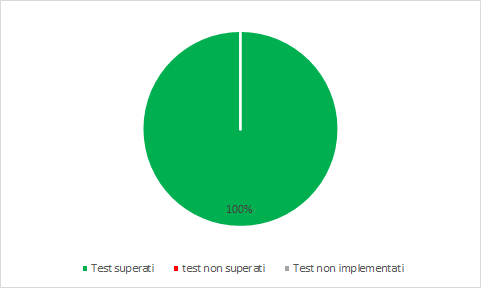
\includegraphics[width=0.6\textwidth]{Images/TI.png}
    	\caption{Sintesi della percentuale di test di integrazione superati}
    	\label{TIZ} 
    \end{figure}
    \paragraph{Tracciamento} \mbox{}
    \newcolumntype{U}{>{\centering\arraybackslash}m{10cm}}
    \begin{longtable}{|c|U|}
    	\hline
    	\textbf{Id Test} & \textbf{Componente}\\
    	\hline
    	\endhead
    	TI1 & Havana \\ \hline
    	TI2 & Client \\ \hline
    	TI3 & Client \\ \hline
    	TI4 & Client \\ \hline
    	TI5 & Client \\ \hline
    	TI6 & Client \\ \hline
    \end{longtable}
	
	\subsubsection{Test di unità}
	\label{TU}
	Lo scopo di questa tipologia di test è di verificare la più piccola parte di lavoro prodotta da un programmatore. Questo significa tendenzialmente verificare i metodi e le funzioni scritte.
	
	\begin{longtable}{|c|H|c|}
		\hline
		\textbf{Id Test} & \textbf{Descrizione} & \textbf{Stato}\\
		\hline
		\endhead
		TU1 & Viene verificato che i dati vengano letti correttamente da \emph{Elasticsearch} & \textcolor{green}{Superato} \\ \hline
		TU2 & Viene verificato che la sorgente dei dati venga impostata correttamente & \textcolor{green}{Superato} \\ \hline
		TU3 & Viene verificato che i dati ottenuti da \emph{Elasticsearch} siano solo quelli contenenti delle trace &\textcolor{green}{Superato} \\ \hline
		TU4 & Viene verificato che i metadati vengano rimossi correttamente da un indice & \textcolor{green}{Superato} \\ \hline
		TU5 & Viene verificato che i metadati vengano rimossi correttamente da un array di indici & \textcolor{green}{Superato} \\ \hline
		TU6 & Viene verificato che i dati utili per la costruzione della mappa topologica vengano puliti correttamente  & \textcolor{green}{Superato} \\ \hline
		TU7 & Viene verificato che i dati utili per la costruzione della stack trace vengano puliti correttamente & \textcolor{green}{Superato} \\ \hline
		TU8 & Viene verificato che la strategia di pulizia dei dati venga impostata correttamente & \textcolor{green}{Superato} \\ \hline
		TU9 & Viene verificato che i campi dati di una trace vengano modificati correttamente se la trace è associata a una richiesta di tipo pageload oppure di tipo database & \textcolor{green}{Superato} \\ \hline
		TU10 & Viene verificato che i call tree vengano trasformati correttamente da stringa ad una gerarchia di oggetti & \textcolor{green}{Superato} \\ \hline
		TU11 & Viene verificato che i tempi di esecuzione delle chiamate siano corretti & \textcolor{green}{Superato} \\ \hline
		TU12 & Viene verificato che non possano essere inseriti due nodi uguali nella mappa topologica & \textcolor{green}{Superato} \\ \hline
		TU13 & Viene verificato che non possano essere inseriti due archi uguali nella mappa topologica & \textcolor{green}{Superato} \\ \hline
		TU14 & Viene verificato che sia possibile ottenere correttamente l'id di un nodo & \textcolor{green}{Superato} \\ \hline
		TU15 & viene verificato che sia possibile ottenere correttamente il link cercato & \textcolor{green}{Superato} \\ \hline
		TU16 & Viene verificato che i nodi vengano aggiunti correttamente alla mappa & \textcolor{green}{Superato} \\ \hline
		TU17 & Viene verificato che gli archi vengano aggiunti correttamente alla mappa & \textcolor{green}{Superato} \\ \hline
		TU18 & Viene verificato che i nodi della mappa vengano costruiti correttamente dato un array di richieste HTTP e a database & \textcolor{green}{Superato} \\ \hline
		TU19 & viene verificato che gli archi della mappa vengano costruiti correttamente dato un array di JSON & \textcolor{green}{Superato} \\ \hline
		TU20 & viene verificato che i nodi del grafo vengano costruiti correttamente & \textcolor{green}{Superato} \\ \hline
		TU21 & viene verificato che le trace vengano costruite correttamente & \textcolor{green}{Superato} \\ \hline
		TU22 & viene verificato che il server ritorni l'indice richiesto con limite e tipo corretti  & \textcolor{green}{Superato} \\ \hline
		TU23 & viene verificato che le richieste vengano suddivise correttamente in base al campo type & \textcolor{green}{Superato} \\ \hline
		TU24 & viene verificato che le singole trace vengano create correttamente & \textcolor{green}{Superato} \\ \hline
		TU25 & viene verificato che venga creato correttamente un oggetto StackTrace & \textcolor{green}{Superato} \\ \hline
		TU26 & viene verificato che dato un array di richieste vengano costruiti correttamente i Links & \textcolor{green}{Superato} \\ \hline
		TU27 & viene verificato che l'oggetto GraphBuilderDirector venga costruito correttamente & \textcolor{green}{Superato} \\ \hline
		
		
		
	\end{longtable}
    
    \begin{figure}[H]
    	\centering 
    	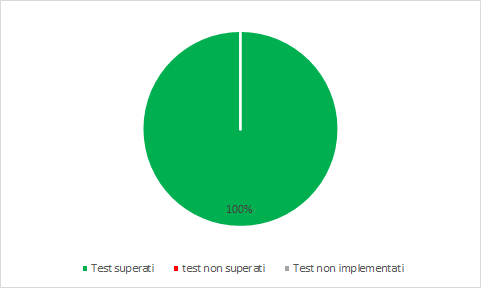
\includegraphics[width=0.6\textwidth]{Images/TU.png}
    	\caption{Sintesi della percentuale di test di unità superati}
    	\label{TUZ} 
    \end{figure}
    
    \paragraph{Tracciamento test di unità-metodi} \mbox{}
    
    \normalsize
    \begin{longtable}{|c|U|}
    	\hline
    	\textbf{Id Test} & \textbf{Metodo}\\
    	\hline
    	\endhead
    	TU1 & Client::dataReader::readData()\newline
    	 Client::dataReader::readIndex() \\ \hline 
    	TU2 & Client::dataReader::setElasticsearchInstance() \\ \hline
    	TU3 & Client::dataReader::tracesIndices() \\ \hline
    	TU4 & Client::dataCleaner::removeMetaDataFromIndex() \\ \hline
    	TU5 & Client::dataCleaner::removeMetaDataFromIndices()\\ \hline
    	TU6 & Client::GraphCleanerStrategy::clean() \\ \hline
    	TU7 & Client::StackCleanerStrategy::Clean()\\ \hline
    	TU8 & Client::dataCleaner::setStrategy()\\ \hline
    	TU9 & Client::Trace::checkPageload()\newline 
    	Client::Trace::checkQueries() \\ \hline
    	TU10 & Client::CallTree::constructor() \newline
    	Client::CallTree::more\_data() \newline
    	Client::CallTree::tableToTree() \\ \hline
    	TU11 & Client::Trace::changeDuration()\\ \hline
    	TU12 & Client::Graph::checkIfNodeIsNotPresent() \\ \hline
    	TU13 & Client::Graph::checkIfLinkIsNotPresent() \\ \hline
    	TU14 & Client::Graph::getIdOfNode() \\ \hline
    	TU15 & Client::Graph::getIndexOfSameLink() \\ \hline
    	TU16 & Client::Graph::addNode() \\ \hline
    	TU17 & Client::Graph::addLink() \\ \hline
    	TU18 & Client::Graph::addNode() \\ \hline
    	TU19 & Client::Graph::addLink() \\ \hline
    	TU20 & Client::GraphBuilder::buildNodes() \\ \hline
    	TU21 & Client::StackBuilder::buildTrace() \\ \hline
    	TU22 & Server::Index::Index() \\ \hline
    	TU23 & Client::StackBuilderDirector::divideRequest() \\ \hline
    	TU24 & Client::StackBuilder::buildTrace() \\ \hline
    	TU25 & Client::StackBuilder::buildTraces() \\ \hline
    	TU26 & Client::GraphBuilder::buildLinks() \\ \hline
    	TU27 & Client::GraphBuilderDirector::constructor() \\ \hline
    \end{longtable}
		
		
	
	
		

	
	
